\chapter{Исследовательская часть}

\section{Технические характеристики}

Технические характеристики устройства, на котором выполнялось тестирование:

\begin{itemize}
	\item Операционная система: Manjaro \cite{manjaro} Linux x86\_64.
	\item Память: 8 GiB.
	\item Процессор: Intel® Core™ i5-8265U\cite{intel}.
\end{itemize}

Тестирование проводилось на ноутбуке, включенном в сеть электропитания. Во
время тестирования ноутбук был нагружен только встроенными приложениями
окружения, окружением, а также непосредственно системой тестирования.

\section{Примеры работы программы}

В данном подразделе представлены примеры работы программы. На рисунке
\ref{img:input} представлен ввод данных. На рисунке \ref{img:output}
представлены результаты работы программы на введенных данных.
\noindent
\begin{figure}[ht!]
\begin{center}
    \begin{minipage}[h]{0.4\linewidth}
        \begin{center}
            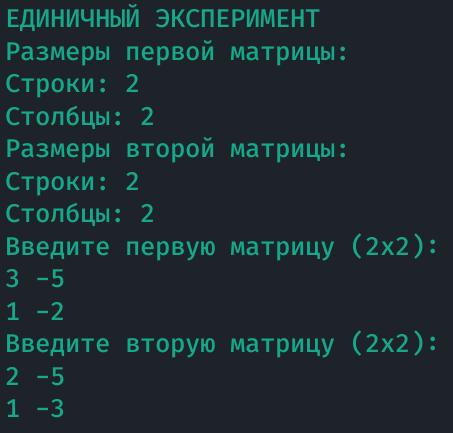
\includegraphics[height=6cm]{../data/img/input.jpg}
            \caption{Пример ввода данных}
            \label{img:input}
        \end{center}
    \end{minipage}
    \hspace{2ex}
    \begin{minipage}[h]{0.4\linewidth}
        \begin{center}
            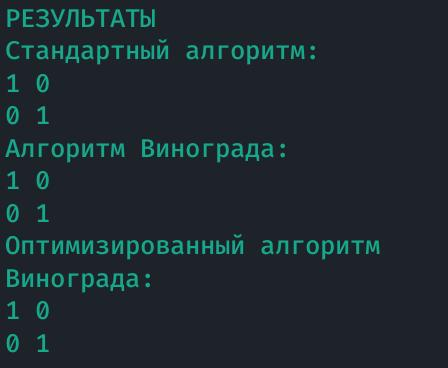
\includegraphics[height=6cm]{../data/img/output.jpg}
            \caption{Пример результата работы программы}
            \label{img:output}
        \end{center}
    \end{minipage}
\end{center}
\end{figure}

\section{Результаты тестирования}

Программа была протестирования на входных данных, приведенных в таблице
\ref{tab:tests}. Полученные результаты работы программы совпали с ожидаемыми
результатами.

\section[Постановка эксперимента по замеру времени]
        {Постановка ~~эксперимента ~~по ~~замеру времени}

Для оценки времени работы релизаций алгоритмов умножения матриц был проведен
эксперимент, в котором определялось влияние размеров матриц на время работы
каждого из алгоритмов. Тестирование проводилось на квадратных матрицах размерами
от 10 до 200 с шагом 10 в начале последовательности и шагом 20 в конце для
исключения ситуации неопределенно долгого ожидания завершения работы программы.
Так как от запуска к запуску процессорное время, затрачиваемое на выполнение
агоритма менялось в определенном промежутке времени, необходимо было усреднить
вычисляемые значения. Для этого каждый алгоритм на каждом значении размера
запускался 10 раз, и для полученных 10 значений определялось среднее
арифметическое, которое и заносилось в таблицу результатов.

Так как в алгоритме Винограда есть зависимость трудоемкости от четности
размера, тестирование также было проведено на последовательности значений
размеров, полученной из выше описанной прибавлением к каждому элементу единицы.

Результаты эксперимента были представлены в виде таблиц и графиков, приведенных
в следующем подразделе.

\section{Результаты эксперимента}

В таблицах \ref{tab:even}, \ref{tab:odd} представлены результаты измерения
времени работы алгоритмов на четных и нечетных размерах матриц соответственно. На
основе табличных данных построены графики зависимости
времени работы каждого алгоритма от размеров матриц (рисунки \ref{img:evenGraph}, \ref{img:oddGraph}).

\begin{table}[h]
	\begin{center}
		\caption{\label{tab:even}Время работы алгоритмов умножения матриц
                 на четных размерах матриц}
		\begin{tabular}{|r|r|r|r|}
			\hline
			\bfseries Размеры  & \bfseries Стандартный&
            \bfseries Винограда & \bfseries\specialcell{ Оптимизированный\\Винограда}
			\csvreader{../data/csv/even.csv}{}
			{\\\hline \csvcoli&\csvcolii&\csvcoliii&\csvcoliv}
			\\\hline
		\end{tabular}
	\end{center}
\end{table}
\noindent
\img{12cm}{evenGraph}{Графики зависимости времени выполнения алгоритмов
умножения матриц от четных размеров матриц}{evenGraph}
\begin{table}[h]
	\begin{center}
		\caption{\label{tab:odd}Время работы алгоритмов умножения матриц
                 на нечетных размерах матриц}
		\begin{tabular}{|r|r|r|r|}
			\hline
			\bfseries Размеры  & \bfseries Стандартный&
            \bfseries Винограда & \bfseries\specialcell{ Оптимизированный\\Винограда}
			\csvreader{../data/csv/odd.csv}{}
			{\\\hline \csvcoli&\csvcolii&\csvcoliii&\csvcoliv}
			\\\hline
		\end{tabular}
	\end{center}
\end{table}
\noindent
\img{12cm}{oddGraph}{Графики зависимости времени выполнения алгоритмов
умножения матриц от нечетных размеров матриц}{oddGraph}

\clearpage
\section{Вывод}

По результатам эксперимента можно сделать следующие выводы:
\begin{itemize}[left=\parindent]
     \item прямая реализация алгоритма Винограда без какой-либо опитимизации
         работает в 1.1 раз медленнее стандартного алгоритма;
     \item оптимизированная версия Винограда работает в 1.2 раз быстрее
         стандартного алгоритма;
     \item при этом оптимизированный алгоритм Винограда работает в 1.05 раза
         быстрее на четных размерах матриц, чем на нечетных.
\end{itemize}

Таким образом, для вычислений произведений матриц при их размерах до 200
следует при необходимости меньшего времени вычислений надо использовать
оптимизированный алгоритм Винограда, при этом предпочтительны четные размеры
матриц, хотя и при нечетных значений оптимизированный алгоритм Винограда дает
выигрыш по времени по сравнению со стандартным.
